\subsection{\bfseries Ažuriranje podataka korisnika od strane korisnika}

\begin{figure}[H]
\begin{center}
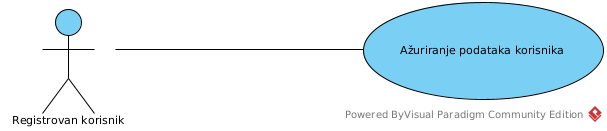
\includegraphics[width=\textwidth]{Pictures/uc_update_user_profile.png}
\end{center}
    \caption{Dijagram slučaja upotrebe ažuriranja podataka korisnika}
\label{fig:UCUpdateUserProfile}
\end{figure}

\begin{itemize}
    \item Kratak opis:
        \begin{itemize}
            \item Registrovani korisnik ažurira svoje podatke putem aplikacije
        \end{itemize}
    \item Učesnici:
        \begin{itemize}
            \item Registrovan korisnik
        \end{itemize}
    \item Preduslovi:
        \begin{itemize}
            \item Sistem je u ispravnom stanju
            \item Korisnik mora biti registrovan i ulogovan na aplikaciju
        \end{itemize}
    \item Postuslovi:
        \begin{itemize}
            \item Podaci su uspešno sačuvani u bazi podataka
        \end{itemize}
    \item Osnovni tok:
        \begin{enumerate}
            \item Korisnik bira opciju da ažurira svoje podatke
            \item Sistem prikazuje formular za izmenu podataka
            \item Korisnik menja željene podatke 
            \item Korisnik bira opciju za čuvanje podataka
            \item Sistem proverava da li su sva polja popunjena
            \item Sistem čuva podatke i prikazuje poruku o uspešnosti
        \end{enumerate}
    \item Alternativni tok:
        \begin{itemize}
            \item Pad sistema. Ukoliko sistem prestane sa radom u bilo kom trenutku, prelazi se na slučaj upotrebe ``Pravljenje rezervne kopije i oporavak baze podataka''.
            \item Ukoliko sistem u 5. koraku pronađe prazno polje, obeležava ga i obaveštava korisnika da sva polja moraju biti popunjena. Korisnik popunjava polje. Proces se nastavlja u 4. koraku osnovnog toka.
        \end{itemize}
    \item Dodatne informacije:
        \begin{itemize}
            \item Podaci koji se mogu menjati su imejl adresa, lozinka i broj platne kartice
        \end{itemize}
\end{itemize}

\begin{figure}[H]
\begin{center}
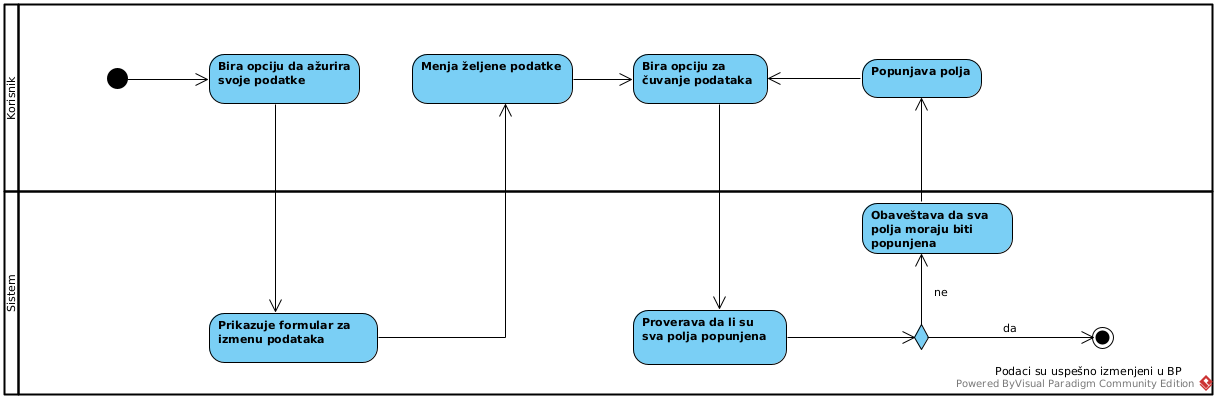
\includegraphics[width=\textwidth]{Pictures/activity_update_user_profile.png}
\end{center}
    \caption{Dijagram aktivnosti ažuriranja podataka korisnika}
\label{fig:ActivityUpdateUserProfile}
\end{figure}
